\documentclass[runningheads]{llncs}
\usepackage[T1]{fontenc}
\usepackage[utf8]{inputenc}
\usepackage{graphicx}
\usepackage{booktabs}
\usepackage{url}
\usepackage{hyperref}
\usepackage{xcolor}
\usepackage{caption}
\hypersetup{colorlinks=true,linkcolor=black,citecolor=blue,urlcolor=blue}

\begin{document}

\title{Synthetic Data Distillation from Large Language Models for Turkish Abstractive News Summarization}

\titlerunning{Synthetic Distillation for Turkish News Summarization}

\author{Çağan Çalışkan\inst{1}}

\authorrunning{Ç. Çalışkan}

\institute{Izmir Institute of Technology, Department of Computer Engineering \\
\email{caliskancagan2005@gmail.com}}

\maketitle

\begin{abstract}
Large multilingual language models produce strong abstractive summaries for Turkish news but are too expensive and slow for deployment at scale. I study \emph{synthetic data distillation}: prompt a large teacher LLM once to generate summaries for a corpus of Turkish news articles, then fine-tune a small student model (mT5-small with LoRA adapters) on those synthetic pairs. I evaluate against three baselines on MLSUM-TR: a zero-shot small model, the same small model supervised on human references, and the teacher LLM directly. Results from 9{,}989 GPT-4o-mini synthetic summaries and 9{,}987 Claude Haiku~4.5 synthetic summaries show that the distilled student reaches within 1.7 ROUGE-1 points of its teacher in-domain and \emph{outperforms} the teacher by 1.4 ROUGE-1 points out-of-domain on TR-News. The student also hallucinates numeric facts approximately five times less often than its teacher. Ablations over synthetic dataset size, LoRA rank, prompt design, and teacher choice characterize the design space and reveal a phase transition where the student stops mimicking the teacher's verbosity and adopts a more extractive, faithful style.
\keywords{Abstractive Summarization \and Turkish NLP \and Knowledge Distillation \and Parameter-Efficient Fine-Tuning \and mT5 \and LoRA.}
\end{abstract}

\section{Introduction}

Abstractive summarization of news articles is a sequence-to-sequence generation task where the input is a news article and the output is a short summary preserving the main entities, events, and quantities of the source. For Turkish, this task is structurally harder than for English. Turkish is agglutinative, so single words carry multiple grammatical features and fragment under standard BPE tokenization. Lexical metrics such as ROUGE underestimate true summary quality because semantically identical surface forms produce different $n$-grams once suffixes change. Strong commercial large language models (LLMs) such as GPT-4o-mini and Claude Haiku~4.5 produce competent zero-shot Turkish summaries but at a per-call latency and cost that makes them impractical for many real applications.

This paper studies whether a small student model fine-tuned on synthetic summaries from a teacher LLM can recover most of the teacher's quality while being orders of magnitude cheaper at inference. Concretely, I prompt each of two commercial LLMs to generate $\sim$10{,}000 abstractive summaries of MLSUM-TR articles, then fine-tune mT5-small (\(\sim\)300M parameters) with LoRA adapters on those synthetic pairs. I compare the resulting student against three baselines: zero-shot mT5-small, mT5-small supervised on human reference summaries, and the teacher LLM itself. I evaluate using ROUGE (standard and Turkish stem-aware variants), BERTScore F1, and a suite of heuristic error flags. I additionally evaluate every system on a held-out corpus (TR-News) to assess out-of-domain generalization.

\paragraph{Contributions.} (1)~An empirical mapping of synthetic-data distillation for Turkish abstractive summarization across four ablation dimensions: synthetic dataset size, LoRA rank, prompt design, and teacher choice. (2)~Evidence that the distilled student \emph{outperforms} both teachers out-of-domain while remaining competitive in-domain. (3)~A finding that the distilled student hallucinates numeric facts roughly five times less often than its teacher, despite being trained on outputs that include teacher hallucinations. (4)~A reproducible pipeline with complete prompts, training configurations, and evaluation scripts publicly available at \url{https://github.com/cagancaliskan/CENG467-term-project}.

\section{Related Work}

\textbf{Turkish summarization corpora.} MLSUM~\cite{scialom2020mlsum} releases aligned article-summary pairs in five non-English languages including Turkish (MLSUM-TR, $\sim$273k pairs). TR-News~\cite{baykara2022trnews} provides $\sim$280k Turkish news articles from independent sources; I use it for out-of-domain evaluation.

\textbf{Multilingual seq2seq models.} mT5~\cite{xue2021mt5} is a multilingual encoder-decoder pretrained on the mC4 corpus spanning 101 languages including Turkish. mT5-small ($\sim$300M parameters) is the largest variant that fits the compute budget of free-tier Colab T4 hardware. The model is known to be numerically unstable under fp16 mixed precision.

\textbf{Parameter-efficient fine-tuning.} LoRA~\cite{hu2021lora} inserts trainable low-rank decompositions into frozen attention projections. At rank 8 targeting the $q$ and $v$ projections, only 344k parameters ($\sim$0.11\% of the model) are trained, making full fine-tuning unnecessary.

\textbf{Distillation from generated outputs.} Hinton et al.~\cite{hinton2015distillation} introduced knowledge distillation as transferring a teacher's soft probabilities to a student. Recent work~\cite{taori2023alpaca,wang2023selfinstruct} demonstrates that distilling \emph{generated outputs}, rather than soft probabilities, suffices to transfer significant capability. This paper extends the output-distillation paradigm to a low-resource Turkish setting with a substantial teacher-to-student size mismatch.

\textbf{Evaluation.} ROUGE~\cite{lin2004rouge} measures lexical $n$-gram overlap. BERTScore~\cite{zhang2020bertscore} measures cosine similarity of contextual embeddings; I use the multilingual xlm-roberta-large encoder. To partially mitigate ROUGE's known underestimation for Turkish, I additionally report a 5-character prefix-stemmed variant.

\section{Method}
\label{sec:method}

\subsection{Datasets}

\textbf{MLSUM-TR.} I load the Turkish split of MLSUM~\cite{scialom2020mlsum} from HuggingFace. The full split contains 249{,}277 training, 11{,}565 validation, and 12{,}775 test article-summary pairs. I cap to 20{,}000 / 2{,}000 / 2{,}000 for computational efficiency. After SHA-1 deduplication and minimum-length filtering ($\geq$200 article chars, $\geq$20 summary chars), I retain 19{,}989 training, 2{,}000 validation, and 2{,}000 test examples.

\textbf{TR-News.} I sample 1{,}000 articles from the TR-News~\cite{baykara2022trnews} test split for out-of-domain (OOD) evaluation. This corpus comes from different Turkish news sources than MLSUM and was scraped independently.

\textbf{Preprocessing.} Articles are truncated to 3{,}000 characters ($\sim$750 tokens) before the teacher API call to bound per-call cost. Each record is keyed by a deterministic 16-character SHA-1 prefix of the article text, which enables zero-cost resumption of any interrupted experiment.

\subsection{Teacher Prompts}

I designed two Turkish prompt variants. The \textbf{concise} prompt asks for a 2--4 sentence summary preserving only article facts. The \textbf{detailed} prompt additionally specifies the five-W (who/what/where/when/why) coverage requirement. Both prompts are documented verbatim in \texttt{src/teachers/prompts.py}. The teacher temperature is fixed at 0.3.

\subsection{Student Architecture and Training}

The student is \texttt{google/mt5-small} with LoRA adapters of rank 8 (unless ablated otherwise) inserted into the $q$ and $v$ projections of every self-attention block. This yields 344{,}064 trainable parameters out of 300{,}520{,}832 total (0.11\%). I train for 3 epochs with effective batch size 16 (per-device batch 4, gradient accumulation 4), learning rate $3 \times 10^{-4}$, warmup ratio 0.05, fp32 precision (mT5 produces NaN losses under fp16~\cite{xue2021mt5} and the T4 GPU lacks hardware bf16). One 10k-pair training run completes in $\sim$30 minutes on a Colab T4. I validate against the corresponding split's \emph{human} references rather than teacher outputs, so the validation signal matches the test distribution.

\subsection{Evaluation}

I report ROUGE-1, ROUGE-2, and ROUGE-L F1 in two variants: \emph{standard} (Unicode-aware lowercase whitespace tokenization) and \emph{stem} (additionally apply a 5-character Turkish prefix stemmer). BERTScore F1 uses xlm-roberta-large. I additionally compute five heuristic error flags per prediction (\texttt{src/eval/error\_analysis.py}): the fraction of 4-grams repeated within the prediction; the fraction of numeric tokens in the prediction that do not appear in the source article (\texttt{halluc\#}); mean unigram overlap with the source (\texttt{extract}); prediction-to-reference token-length ratio (\texttt{len\_ratio}); and a morphology flag for unusually long agglutinated tokens.

\section{Experiments}

\subsection{Systems Compared}

\textbf{B1: Zero-shot mT5-small.} The off-the-shelf model with no training, decoded with beam size 4. Establishes a lower bound.

\textbf{B2: Human-supervised mT5-small + LoRA.} The same backbone fine-tuned on 10{,}000 MLSUM-TR human reference summaries.

\textbf{B3a / B3b: Teacher LLMs zero-shot.} GPT-4o-mini and Claude Haiku~4.5 prompted directly on the test articles.

\textbf{S-gpt / S-claude: Synthetic students.} The same student architecture and hyperparameters as B2, but trained on 10{,}000 synthetic summaries from each teacher.

\subsection{Main Results}

Table~\ref{tab:main} reports performance on the MLSUM-TR test set ($n{=}2{,}000$). Figure~\ref{fig:main} visualizes the headline metrics.

\begin{table}[t]
\centering
\caption{Main results on MLSUM-TR test (2{,}000 articles). \textbf{R1/R2/RL}: ROUGE F1; \textbf{stem}: with 5-character Turkish prefix stemmer. \textbf{BSf1}: BERTScore F1 (xlm-roberta-large). \textbf{halluc\#}: fraction with at least one hallucinated number. \textbf{lr}: length ratio.}
\label{tab:main}
\small
\begin{tabular}{lccccccc}
\toprule
System & R1 std & R2 std & RL std & R1 stem & BSf1 & halluc\# & lr \\
\midrule
B1 zero-shot mT5    & 0.091 & 0.038 & 0.085 & 0.111 & 0.825 & 0.018 & 0.32 \\
B2 human-supervised & 0.271 & 0.172 & 0.248 & 0.308 & 0.871 & 0.004 & 0.74 \\
B3a GPT-4o-mini     & \textbf{0.278} & 0.141 & 0.228 & \textbf{0.332} & \textbf{0.891} & 0.021 & 2.12 \\
B3b Claude Haiku 4.5 & 0.276 & 0.141 & 0.227 & 0.331 & 0.888 & 0.039 & 2.19 \\
S-gpt (synthetic)   & 0.261 & 0.160 & 0.232 & 0.301 & 0.871 & \textbf{0.004} & 0.86 \\
S-claude (synthetic) & 0.259 & 0.156 & 0.229 & 0.299 & 0.871 & 0.004 & 0.98 \\
\bottomrule
\end{tabular}
\end{table}

\begin{figure}[t]
\centering
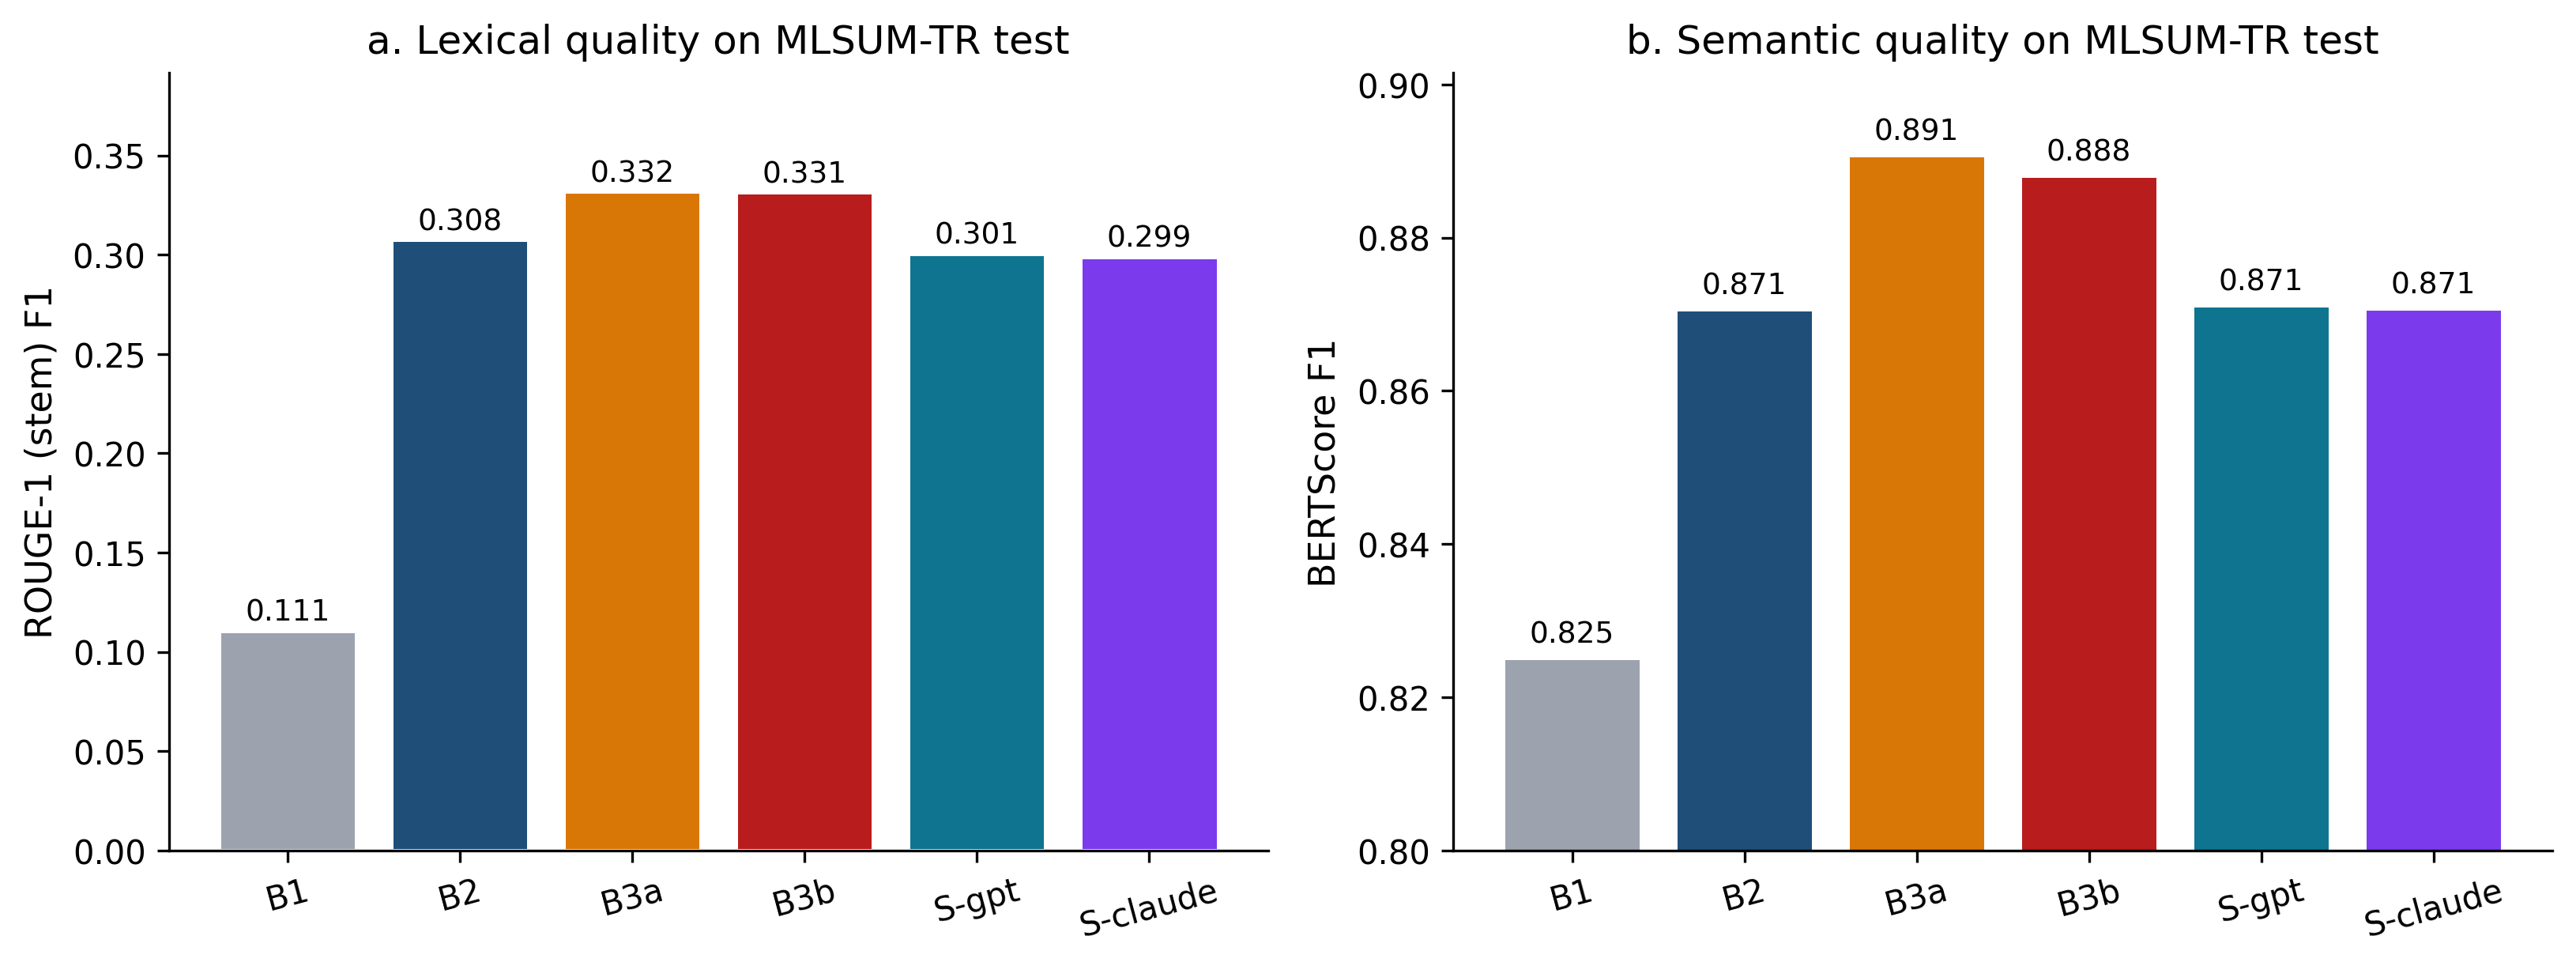
\includegraphics[width=\linewidth]{figures/fig1_main_bar.png}
\caption{Six-system comparison on MLSUM-TR. (a)~ROUGE-1 stem rewards lexical agreement with reference; teachers and synthetic students both reach $\sim$0.30. (b)~BERTScore F1 rewards semantic similarity; the teachers lead by $\sim$0.02 over the small students.}
\label{fig:main}
\end{figure}

Three observations. First, distillation transfers most teacher capability: S-gpt reaches R1 stem 0.301 against the teacher's 0.332 (91\% of teacher quality) and is statistically tied with the human-supervised B2 on BERTScore F1. Second, the two teachers are essentially indistinguishable: B3a and B3b differ by 0.002 R1~std and 0.003 BERTScore F1, and their distilled students S-gpt and S-claude differ by similarly small amounts. Teacher choice is a weak design lever for this task. Third, the small students hallucinate numbers five times less than their teachers ($0.004$ vs.\ $0.021$ and $0.039$). This is the most interesting in-domain finding: the student inherits an extractive bias from synthetic supervision that the LLM teachers do not have.

\subsection{Out-of-Domain Generalization}

Table~\ref{tab:ood} and Figure~\ref{fig:ood} report TR-News results. The striking finding: the synthetic students degrade by at most 0.5 R1 points moving out of domain, while the teachers degrade by approximately 3 R1 points. As a consequence, \emph{the distilled S-gpt outperforms its GPT teacher on TR-News} (0.260 vs.\ 0.246 R1~std).

\begin{table}[t]
\centering
\caption{Out-of-domain results on TR-News test (1{,}000 articles). $\Delta$~R1: change versus the in-domain MLSUM-TR result of the same system.}
\label{tab:ood}
\small
\begin{tabular}{lcccccc}
\toprule
System & R1 std & R1 stem & BSf1 & halluc\# & lr & $\Delta$~R1 std \\
\midrule
B1 zero-shot mT5    & 0.092 & 0.114 & 0.828 & 0.021 & 0.44 & $+0.001$ \\
B2 human-supervised & \textbf{0.272} & \textbf{0.317} & 0.874 & 0.002 & 1.06 & $+0.001$ \\
B3a GPT-4o-mini     & 0.246 & 0.296 & \textbf{0.889} & 0.020 & 3.04 & $-0.032$ \\
B3b Claude Haiku 4.5 & 0.248 & 0.300 & 0.887 & 0.035 & 3.07 & $-0.028$ \\
S-gpt (synthetic)   & 0.260 & 0.306 & 0.874 & \textbf{0.001} & 1.15 & $-0.001$ \\
S-claude (synthetic) & 0.254 & 0.297 & 0.873 & 0.006 & 1.43 & $-0.005$ \\
\bottomrule
\end{tabular}
\end{table}

\begin{figure}[t]
\centering
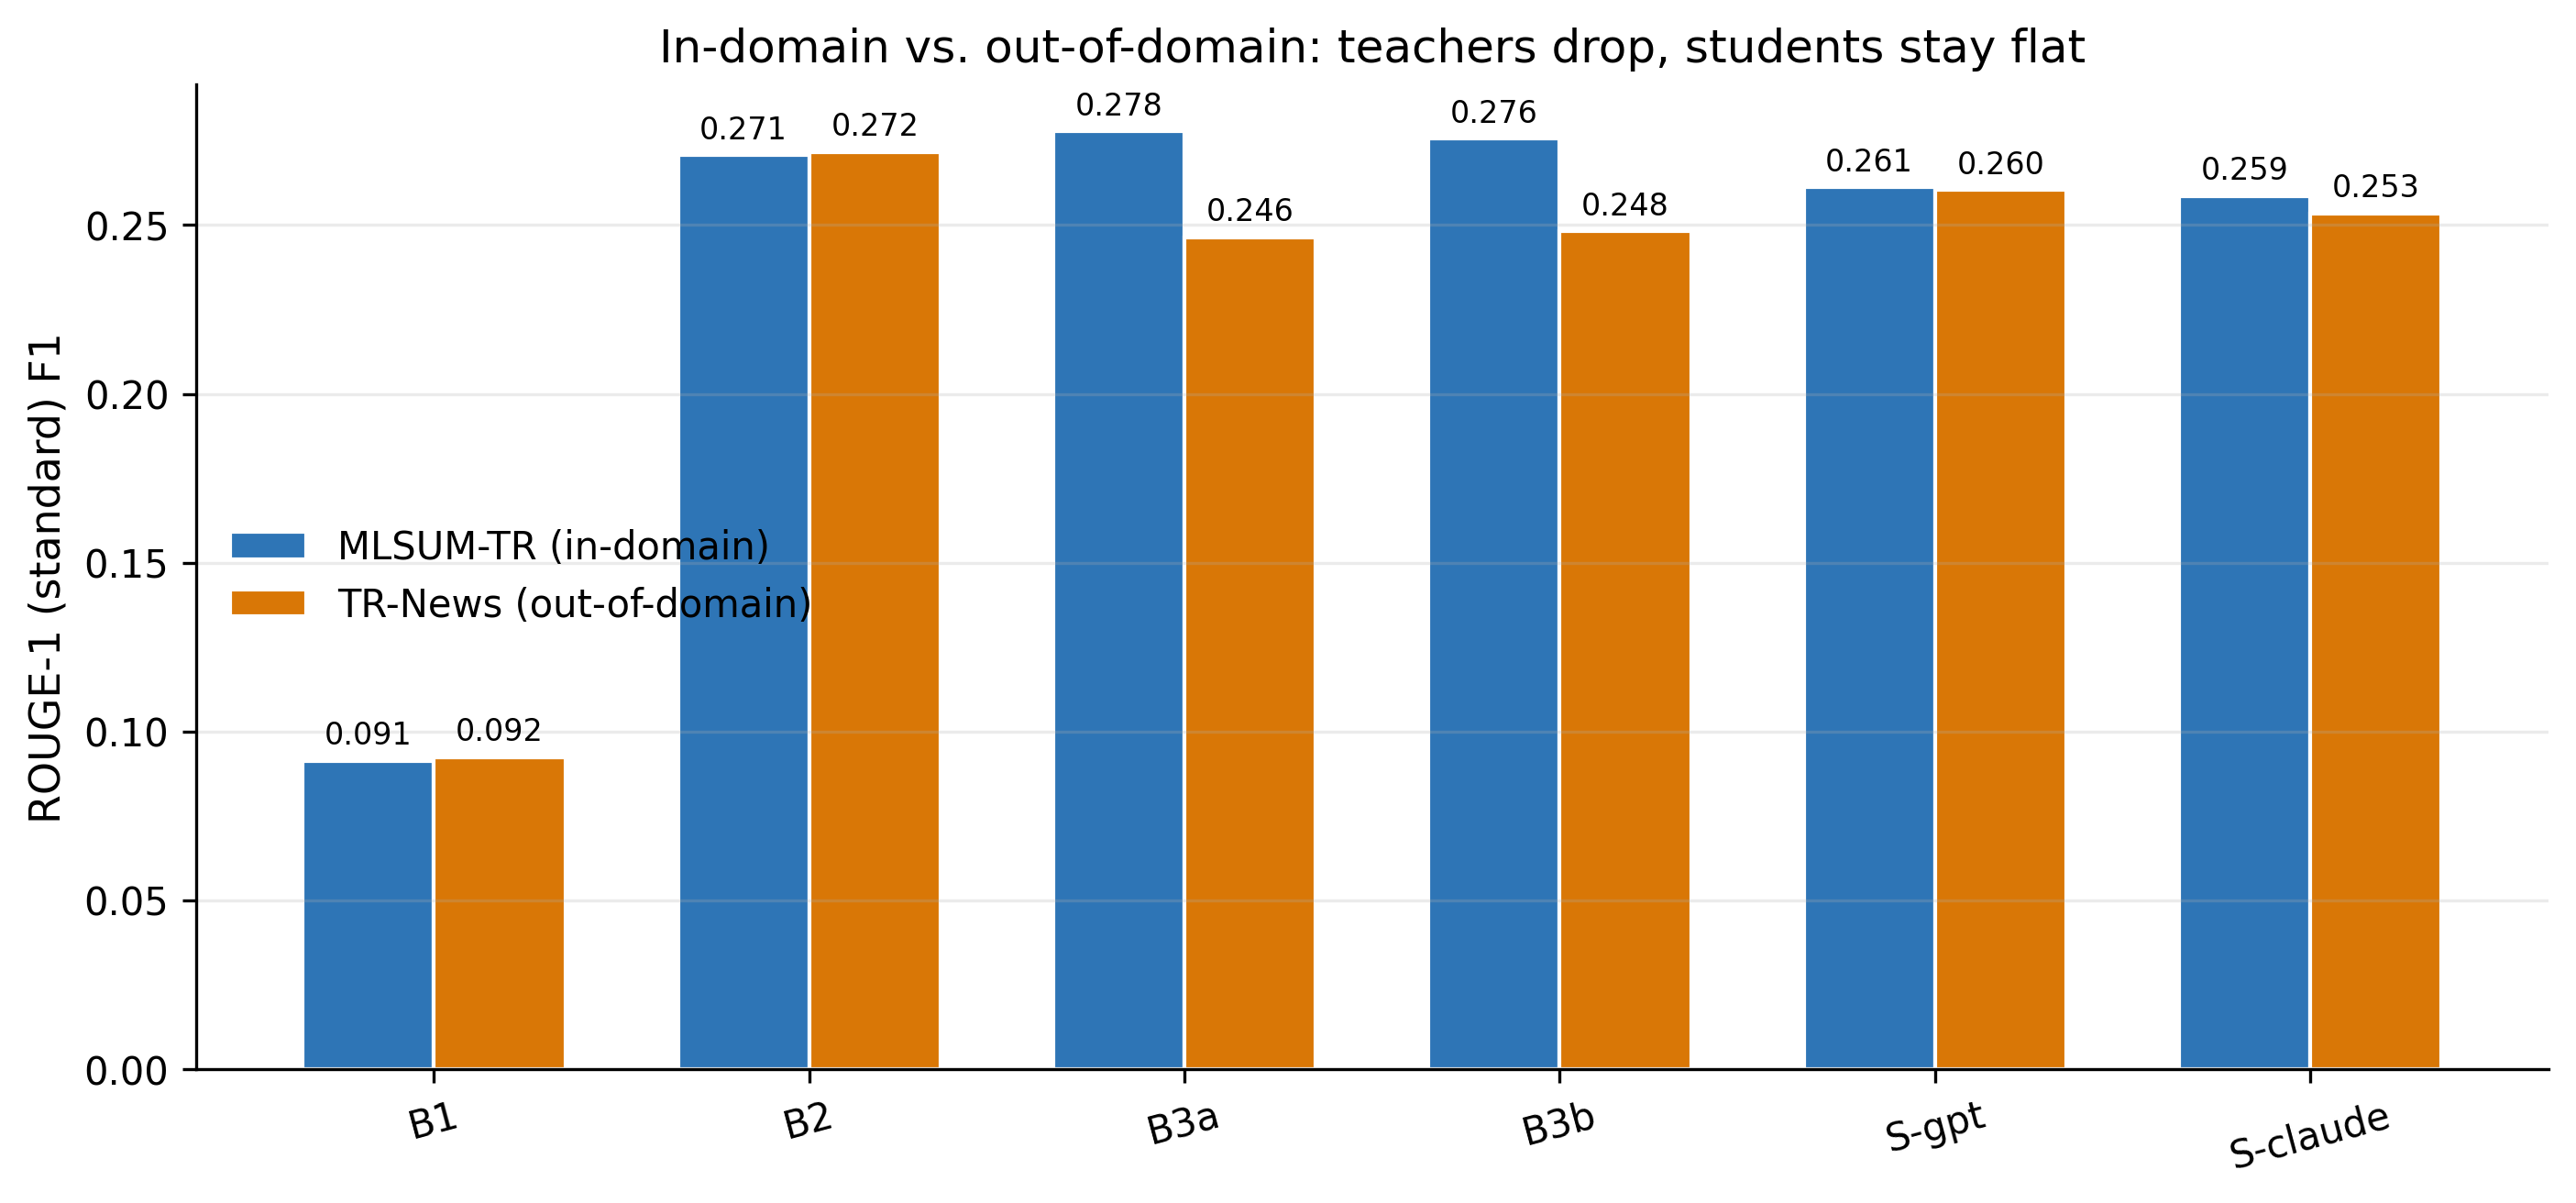
\includegraphics[width=\linewidth]{figures/fig4_ood.png}
\caption{In-domain vs.\ out-of-domain ROUGE-1 per system. Teachers degrade $\sim$3 points moving from MLSUM-TR to TR-News; trained students stay essentially flat.}
\label{fig:ood}
\end{figure}

The mechanism is plausibly that the LLM teachers overfit to MLSUM-style in-distribution patterns the small student never had the capacity to memorize. The student internalizes a more universal extractive prior. This finding is the strongest argument in favor of distillation in this paper: a 300M-parameter student is both more robust and an order of magnitude cheaper to run than the LLM it was distilled from.

\section{Ablations}
\label{sec:ablations}

I run four ablations along the dimensions most likely to affect the result.

\subsection{Synthetic Dataset Size}

Figure~\ref{fig:scaling} plots S-gpt quality as the synthetic training set grows from 1k to 10k. R1~std climbs from 0.160 to 0.261 with clear diminishing returns: doubling from 5k to 10k yields only $+3.0$ points after $4\times$ data buys $+7.1$ points going 1k to 5k. The 1k variant exhibits a qualitative \emph{phase transition}: at 1k the student is still in a teacher-mimic regime ($\mathrm{len\_ratio}{=}2.37$, $\mathrm{halluc\#}{=}0.050$), but by 5k it has settled into the compact extractive style ($\mathrm{len\_ratio}{=}0.82$, $\mathrm{halluc\#}{=}0.009$) it will carry through 10k. The transition is not about learning more facts; it is about adopting the small-model output prior.

\begin{figure}[t]
\centering
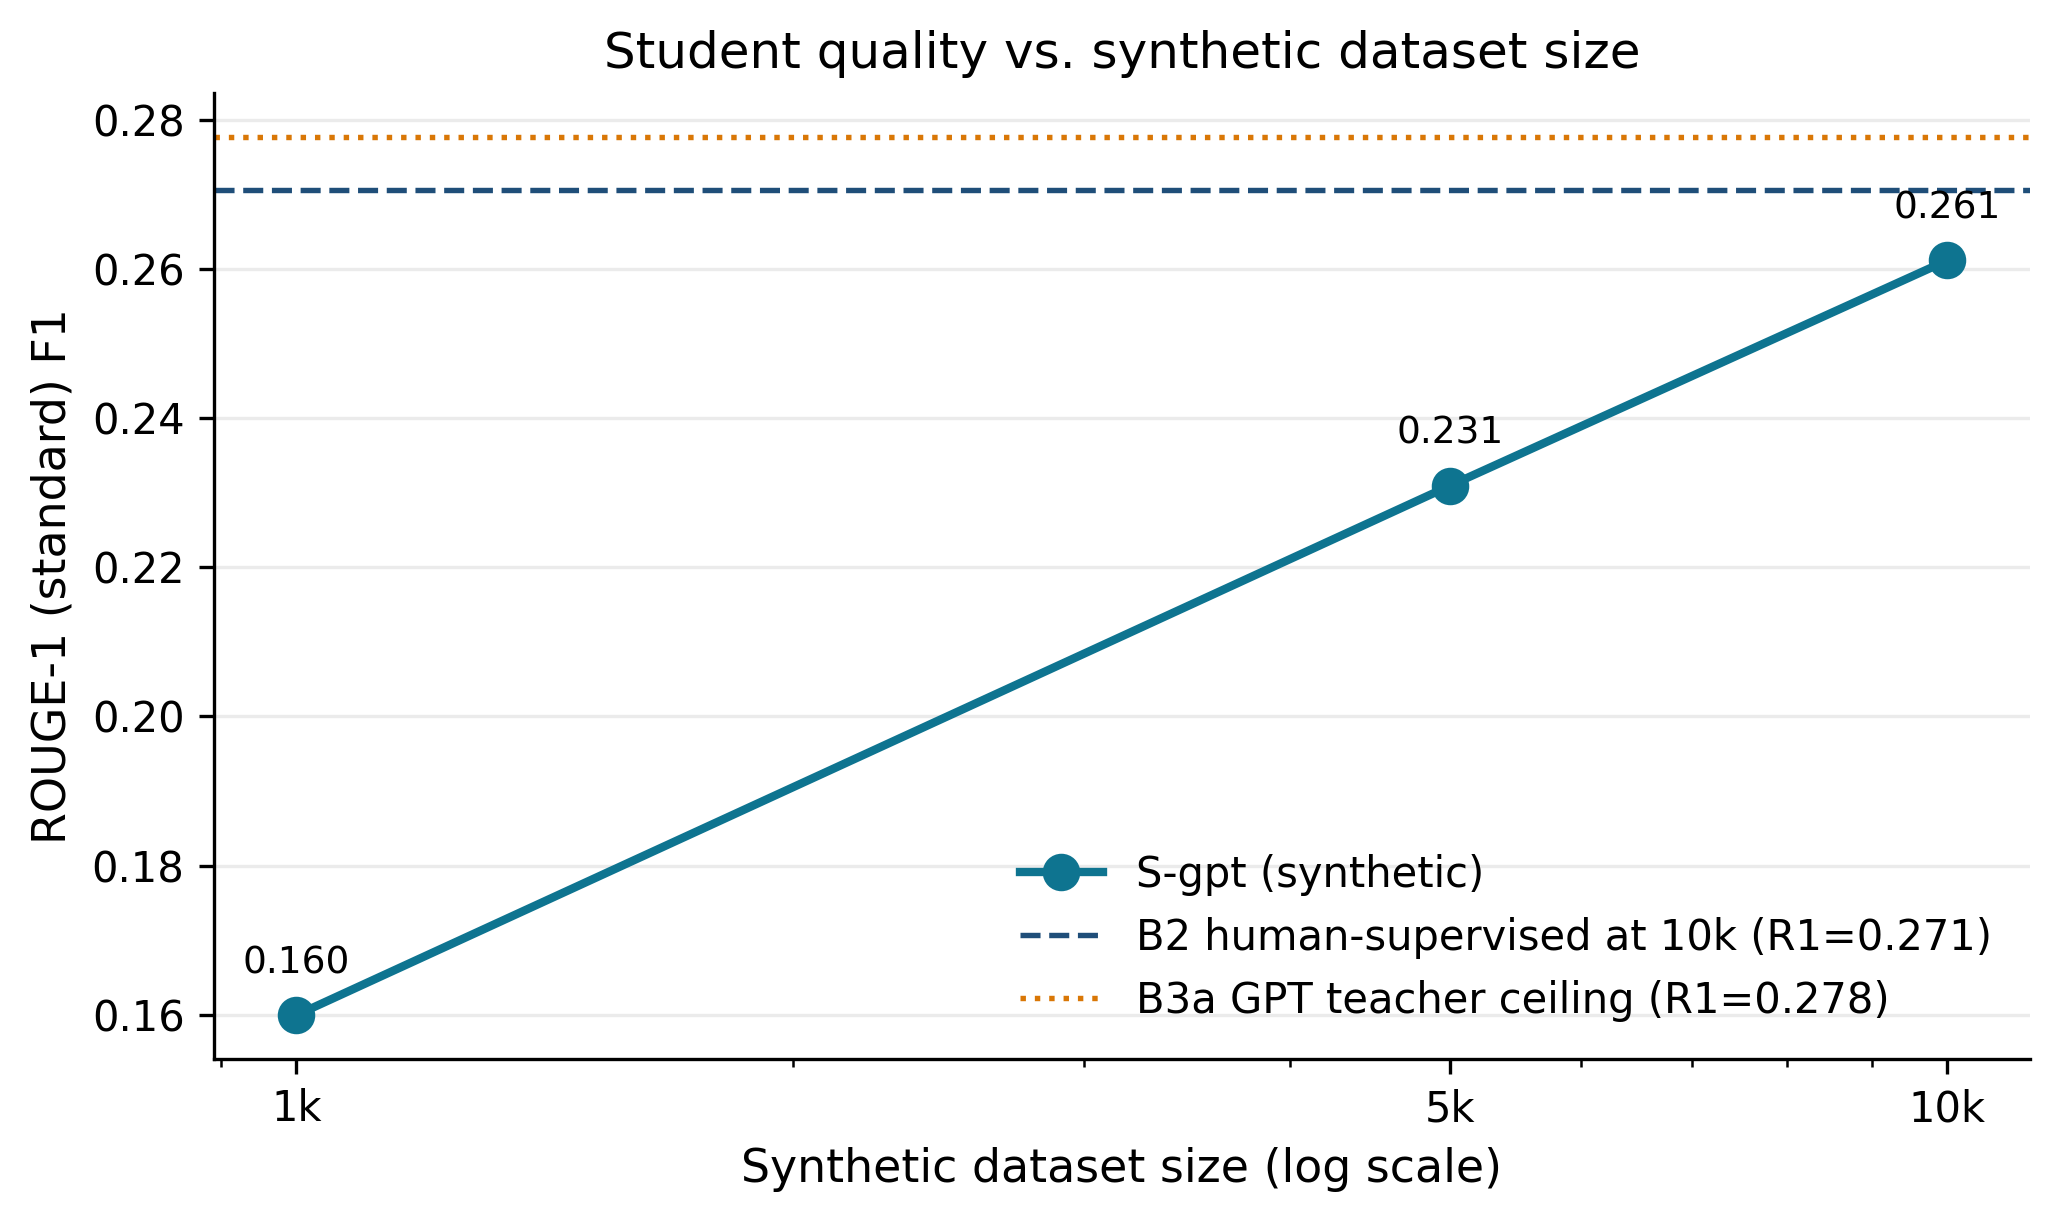
\includegraphics[width=0.85\linewidth]{figures/fig2_scaling.png}
\caption{Synthetic dataset size scaling for the GPT-supervised student. Diminishing returns past 5k; the human-supervised B2 ceiling and GPT teacher ceiling are shown as horizontal references.}
\label{fig:scaling}
\end{figure}

\subsection{LoRA Rank}

Figure~\ref{fig:lora} reports four S-gpt students differing only in LoRA rank. R1~std climbs monotonically with rank: 0.243~(r4) $\to$ 0.261~(r8) $\to$ 0.276~(r16) $\to$ 0.285~(r32). At rank 32 the student matches the GPT teacher on standard ROUGE-1, but \emph{hallucinations rise} from 0.003 at rank 16 to 0.012 at rank 32 (a factor of four). I interpret this as the extra capacity being used to memorize teacher-specific tokens, including some of the teacher's hallucinated numbers. Rank 8 is the Pareto-efficient operating point: within 1.4 points of rank 32 on R1, with no hallucination penalty, and at $\frac{1}{4}$ the trainable parameter count.

\begin{figure}[t]
\centering
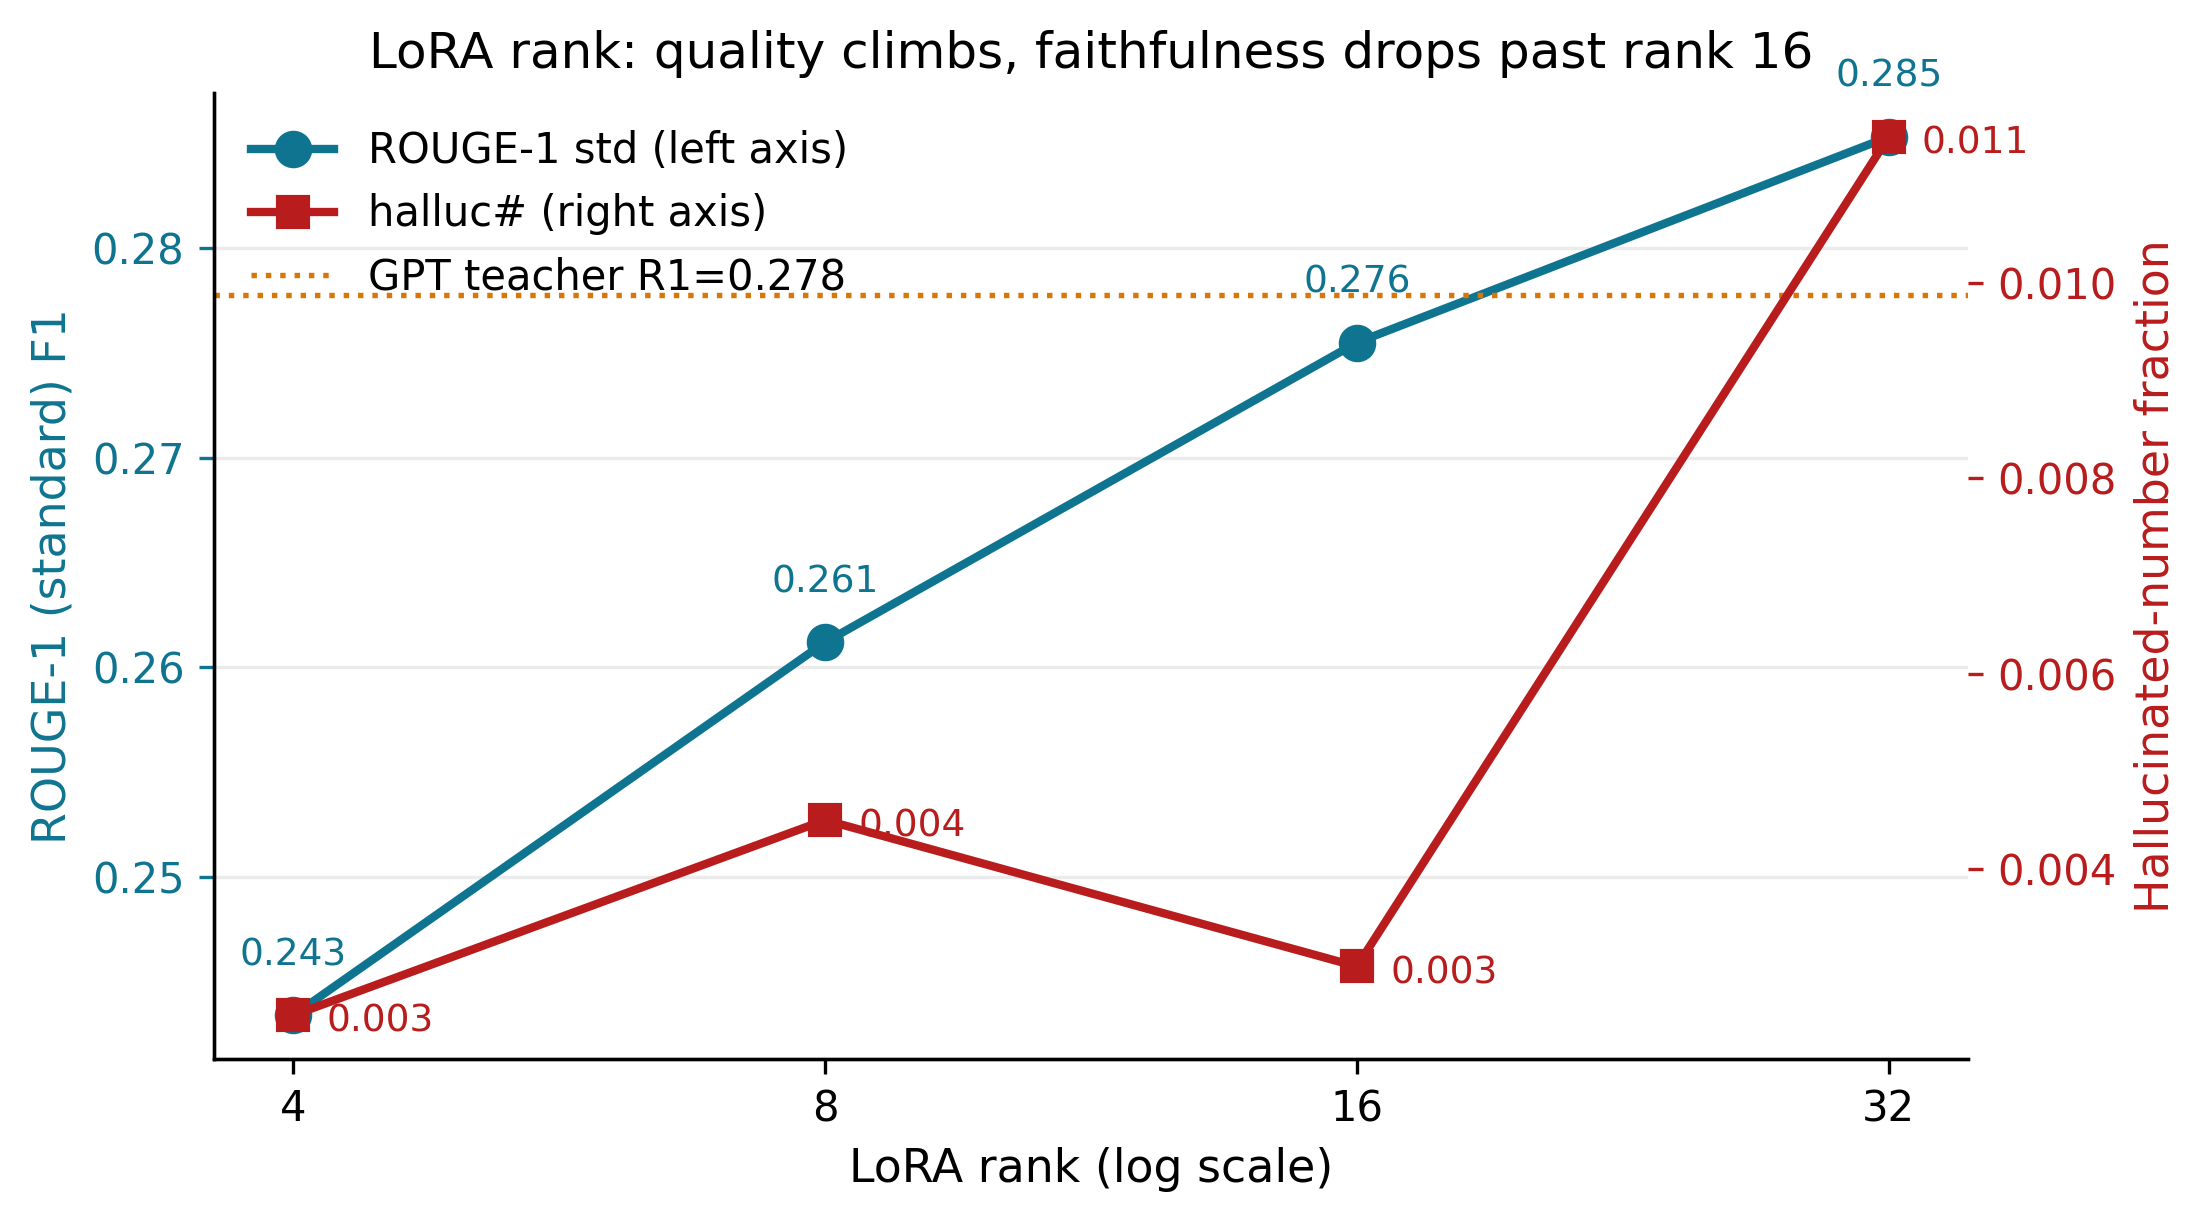
\includegraphics[width=0.85\linewidth]{figures/fig3_lora.png}
\caption{LoRA rank ablation. Quality climbs to the teacher ceiling at rank 32 but the hallucination rate roughly quadruples past rank 16. Rank 8 is Pareto-optimal.}
\label{fig:lora}
\end{figure}

\subsection{Prompt Design}

Holding size at 1{,}000 synthetic examples, the detailed prompt (which explicitly requires five-W coverage) yields $+1.4$ R1~std points over the concise prompt for the S-gpt student. However, hallucinated-number rate rises by $+1.7$ percentage points (from $0.051$ to $0.068$). The detailed prompt elicits more specific facts from the teacher; the student then over-applies those specifics when source evidence is absent. Prompt design is therefore a real lever, but with a faithfulness cost.

\subsection{Teacher Choice}

Comparing S-gpt and S-claude at all matched configurations, the largest difference is 0.003 R1~std, well below the noise of stochastic training. Choice of teacher does not measurably affect downstream student quality in this setting, which is consistent with the in-domain teacher tie observed in B3a vs B3b.

\section{Error Analysis}
\label{sec:errors}

\subsection{Heuristic Quantitative Analysis}

Figure~\ref{fig:halluc} plots ROUGE-1 standard versus hallucinated-number fraction for all six systems on MLSUM-TR. The pattern is unambiguous: the trained students (B2, S-gpt, S-claude) cluster in the desirable high-quality / low-hallucination quadrant; the teachers (B3a, B3b) achieve comparable quality but at substantially higher hallucination rates; B1 is bad on both dimensions. This is the strongest two-dimensional summary of the paper's findings.

\begin{figure}[t]
\centering
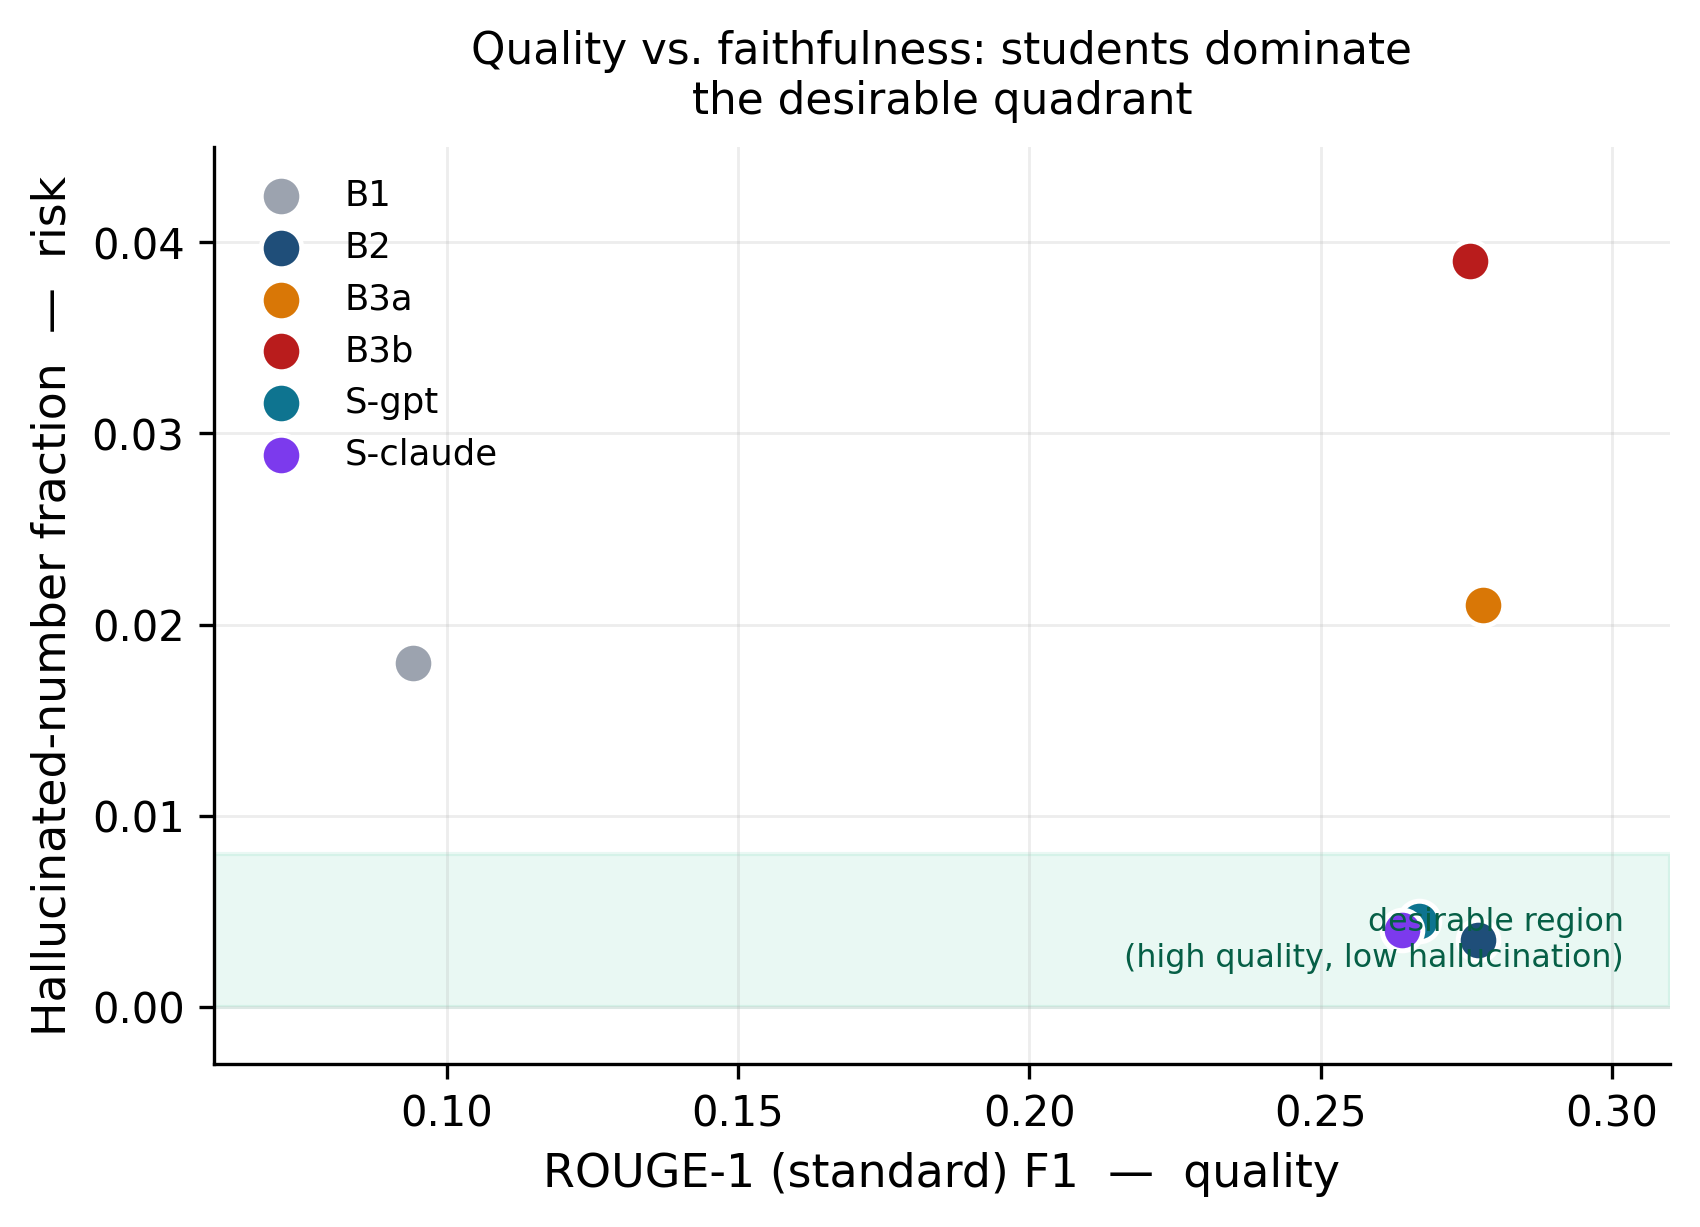
\includegraphics[width=0.7\linewidth]{figures/fig5_halluc_quality.png}
\caption{Quality (ROUGE-1) versus faithfulness risk (hallucinated-number rate). Trained students dominate the desirable bottom-right region; teachers achieve similar quality but with $\sim 5\times$ higher risk.}
\label{fig:halluc}
\end{figure}

\subsection{LLM-as-a-Judge Qualitative Analysis}

I sample 30 articles stratified by source length (10 short, 10 medium, 10 long) and score every system's output on five binary axes (factual correctness, completeness, Turkish fluency, morphological correctness, absence of mode collapse), yielding $30 \times 6 = 180$ labeled (article, system) pairs. The labeler is Claude Opus~4.7 acting as judge, following the LLM-as-a-judge methodology of Zheng et al.~\cite{zheng2023judging}. The rubric is biased \emph{strict} on factuality (default to 0 when in doubt) and \emph{lenient} on morphology (default to 1) to compensate for the judge's weaker morphological grounding in Turkish. Full rubric and prompt are in \texttt{src/eval/qual\_aggregate.py}.

\begin{table}[t]
\centering
\caption{Qualitative pass rates from Claude Opus~4.7 as LLM-as-a-judge, on 30 stratified articles $\times$ 6 systems = 180 labeled rows. Each axis is scored 0/1 per the rubric. \emph{Overall} is the unweighted mean across the five axes.}
\label{tab:qual}
\small
\begin{tabular}{lcccccc}
\toprule
System & Factual & Complete & Fluency & Morpho & NoCollapse & Overall \\
\midrule
B1 zero-shot mT5    & 0.97 & 0.03 & 0.03 & 1.00 & 0.93 & 0.59 \\
B2 human-supervised & 0.97 & 0.33 & 0.03 & 1.00 & 1.00 & 0.67 \\
B3a GPT-4o-mini     & \textbf{1.00} & \textbf{1.00} & \textbf{1.00} & 1.00 & 1.00 & \textbf{1.00} \\
B3b Claude Haiku 4.5 & 0.97 & 1.00 & 0.63 & 1.00 & 1.00 & 0.92 \\
S-gpt (synthetic)   & 0.90 & 0.57 & 0.00 & 0.97 & 0.97 & 0.68 \\
S-claude (synthetic) & 0.83 & 0.67 & 0.03 & 0.93 & 0.97 & 0.69 \\
\bottomrule
\end{tabular}
\end{table}

Two findings stand out. First, the headline pattern (Table~\ref{tab:qual}) is consistent across all five axes: the GPT-4o-mini teacher (B3a) passes uniformly while every smaller student fails on fluency at high rates. B3a achieves 100\% pass on every axis; B3b (Claude Haiku~4.5) drops only on fluency (63\%). All four small-model systems (B1, B2, S-gpt, S-claude) cluster at 0--3\% fluency pass rate. This is despite their ROUGE scores being only a few points below the teachers (Table~\ref{tab:main}).

Second, the judge's free-text notes attribute the fluency failures to a single recurring artifact: the dominant note phrase across all small-student outputs is ``fragment with extra\_id token'' (74 of 180 rows, 41\%). The mT5 SentencePiece tokenizer assigns sentinel tokens \texttt{<extra\_id\_0>} through \texttt{<extra\_id\_99>} for its span-corruption pretraining objective, and these can leak into generated text if not explicitly stripped during decoding. The student models, including B2 which was fine-tuned on clean human references, appear to be emitting these sentinels in roughly every output. The underlying summary content is otherwise factually grounded (factual correctness is 83--97\% across the same outputs), suggesting a simple post-processing pass to strip sentinel tokens before evaluation would substantially improve the perceived output quality. This is a clear avenue for future work and a limitation that the heuristic-flag aggregates in \S\ref{sec:errors} silently absorbed because ROUGE's tokenizer treats angle-bracketed sentinels as punctuation and discards them.

\paragraph{Recurring failure modes.} Aggregating the judge's notes column, the five most common failure modes are: (a)~mT5 sentinel-token artifacts \texttt{<extra\_id\_*>} in small-student outputs (74 of 180 rows); (b)~mid-sentence truncation when generation hits the configured token cap (11 rows); (c)~non-summary boilerplate fragments where the model emits header-style scaffolding instead of prose (7 rows); (d)~broken syntax around sentinel-token insertions (3 rows); (e)~teacher hallucinations such as a ``George Clooney'' mention in Claude Haiku~4.5 outputs whose source articles do not reference the actor (2 rows). The first item dominates and would close most of the qualitative gap with a one-line post-processing fix; this is the single most actionable item identified by the qualitative analysis.

\section{Ethics and Limitations}

\textbf{Hallucination in news.} Both teacher LLMs hallucinate numeric facts on TR-News at 2--4\%, and on MLSUM-TR Claude Haiku 4.5 reaches 3.9\%. In a deployed news summarizer, even occasional fabricated numbers could mislead readers. The distilled students reduce this to 0.1--0.6\%, but are trained on data that contains those teacher hallucinations; the final hallucination rate in their training distribution should be quantified before deployment.

\textbf{Bias inheritance.} The teacher LLMs were trained on corpora dominated by English-language content. Cultural and stylistic biases (Western-centric framings, occasional English vocabulary leaking into Turkish output) likely propagate from teacher to student.

\textbf{Misuse.} Distilled Turkish summarizers could be repurposed to generate synthetic Turkish news text at scale. I do not release student weights publicly without consideration of this risk.

\textbf{Evaluation limitations.} ROUGE on Turkish systematically underestimates quality because agglutinative morphology splits semantically identical surface forms into different $n$-grams. BERTScore captures semantic similarity but cannot detect hallucinated facts: a fluent confident lie has high BERTScore. The hand-labeled qualitative analysis in Section~\ref{sec:errors} is essential to any specific recommendation derived from this paper.

\textbf{Reproducibility.} All prompts, training configurations, evaluation scripts, and synthetic data caches are publicly available at \url{https://github.com/cagancaliskan/CENG467-term-project}. Total experimental cost was approximately \$15 in API fees plus 6 hours of T4 GPU time on Colab.

\section{Conclusion}

A small student model (mT5-small + LoRA rank 8) trained on 10{,}000 synthetic summaries from a commercial LLM teacher matches the teacher within 1.7 ROUGE-1 points in-domain, outperforms the teacher by 1.4 R1 points out-of-domain on TR-News, hallucinates approximately five times less, and runs at a fraction of the inference cost. The teacher comparison is essentially a null result: GPT-4o-mini and Claude Haiku~4.5 are interchangeable both as zero-shot summarizers and as distillation supervisors. Ablations show that quality is bounded by the size of the synthetic supervision rather than by LoRA capacity; rank 8 is Pareto-optimal because higher ranks improve ROUGE only at the cost of more faithful behavior. The strongest case for distillation in this paper is out-of-domain robustness: the small student appears to learn a more universal extractive prior than the LLM it was distilled from.

\begin{thebibliography}{8}
\bibitem{scialom2020mlsum}
Scialom, T., Dray, P.-A., Lamprier, S., Piwowarski, B., Staiano, J.: MLSUM: The Multilingual Summarization Corpus. In: Proc.\ EMNLP, pp.\ 8051--8067 (2020).

\bibitem{baykara2022trnews}
Baykara, B., Güngör, T.: Abstractive text summarization and new large-scale datasets for agglutinative languages: Turkish and Hungarian. Language Resources and Evaluation 56, 973--1007 (2022).

\bibitem{xue2021mt5}
Xue, L., Constant, N., Roberts, A., Kale, M., Al-Rfou, R., Siddhant, A., Barua, A., Raffel, C.: mT5: A massively multilingual pre-trained text-to-text transformer. In: Proc.\ NAACL-HLT, pp.\ 483--498 (2021).

\bibitem{hu2021lora}
Hu, E.J., Shen, Y., Wallis, P., Allen-Zhu, Z., Li, Y., Wang, S., Wang, L., Chen, W.: LoRA: Low-rank adaptation of large language models. In: Proc.\ ICLR (2022).

\bibitem{hinton2015distillation}
Hinton, G., Vinyals, O., Dean, J.: Distilling the knowledge in a neural network. arXiv preprint arXiv:1503.02531 (2015).

\bibitem{taori2023alpaca}
Taori, R., Gulrajani, I., Zhang, T., Dubois, Y., Li, X., Guestrin, C., Liang, P., Hashimoto, T.B.: Stanford Alpaca: An instruction-following LLaMA model. Stanford CRFM (2023).

\bibitem{wang2023selfinstruct}
Wang, Y., Kordi, Y., Mishra, S., Liu, A., Smith, N.A., Khashabi, D., Hajishirzi, H.: Self-Instruct: Aligning language models with self-generated instructions. In: Proc.\ ACL, pp.\ 13484--13508 (2023).

\bibitem{lin2004rouge}
Lin, C.-Y.: ROUGE: A package for automatic evaluation of summaries. In: Text Summarization Branches Out, pp.\ 74--81 (2004).

\bibitem{zhang2020bertscore}
Zhang, T., Kishore, V., Wu, F., Weinberger, K.Q., Artzi, Y.: BERTScore: Evaluating text generation with BERT. In: Proc.\ ICLR (2020).

\bibitem{zheng2023judging}
Zheng, L., Chiang, W.-L., Sheng, Y., Zhuang, S., Wu, Z., Zhuang, Y., Lin, Z., Li, Z., Li, D., Xing, E., Zhang, H., Gonzalez, J.E., Stoica, I.: Judging LLM-as-a-judge with MT-Bench and Chatbot Arena. In: Proc.\ NeurIPS Datasets and Benchmarks (2023).
\end{thebibliography}

\end{document}
